\documentclass[12pt]{article}

\usepackage{comment}

\usepackage{graphicx}

\usepackage[toc,page]{appendix}

\usepackage{titling}
\usepackage{lipsum}
\usepackage{caption}
\usepackage{xcolor}
\usepackage{threeparttable}
\usepackage[numbers]{natbib}
\definecolor{RefColor}{rgb}{0,0,.65}
\usepackage[colorlinks,linkcolor=RefColor,citecolor=RefColor,urlcolor=RefColor]{hyperref}
\usepackage{url}
\def\UrlBreaks{\do\/\do-}
\usepackage{breakurl}
\usepackage{chngcntr}
\usepackage{tikz} 

\usepackage[T1]{fontenc}
\usepackage[utf8]{inputenc}
\usepackage{tabularx,ragged2e,booktabs,caption}
\newcolumntype{C}[1]{>{\Centering}m{#1}}
\renewcommand\tabularxcolumn[1]{C{#1}}

\usepackage{bbm}


\usepackage{amsfonts}
\usepackage{amsmath}
\usepackage{subfloat}
\usepackage{float}
\usepackage[parfill]{parskip}


\usepackage{amsthm}
\newtheorem{definition}{Definition}
\newtheorem{theorem}{Theorem}




\usepackage[font=footnotesize,labelformat=simple]{subcaption}
\renewcommand\thesubfigure{(\alph{subfigure})}

\usepackage{array}
\usepackage{booktabs} % For improved table lines
\renewcommand{\arraystretch}{1.3} % Increase row spacing
\renewcommand{\thesection}{\arabic{section}}
\addtolength{\oddsidemargin}{-.75in}%
\addtolength{\evensidemargin}{-.75in}%
\addtolength{\textwidth}{1.5in}%
\addtolength{\textheight}{1.3in}%
\addtolength{\topmargin}{-.8in}%



\bibliographystyle{unsrtnat}







\title{Comparison of Hakwes Model and Compartmental Models for COVID-19}
\author{Sarah Masri}
\date{\today}

\begin{document}

\maketitle


\thispagestyle{empty}

\begin{abstract}
\noindent  
\end{abstract}





\pagebreak
\section{Background}


The occurrence of pandemics and the spread of infectious disease has induced the application of various epidemiological models to understand and predict the illnesses patterns and behaviour. Among these, the Hawkes model and compartmental models, such as the SIR (Susceptible-Infectious-Recovered) model, stand out as prominent approaches, each with unique characteristics, assumptions and conclusions. Within the application of modelling the spread of SARS-CoV-2, most approaches involve some extension of the classic SIR model~\cite{Garetto2021}.

%The Hawkes model, a type of self-exciting point process, emphasizes the role of temporal clustering in contagion events, effectively capturing the ripple effects of infections over time. In contrast, the SIR model, a compartmental model in epidemiology, classifies the population into distinct groups (susceptible, infectious, and recovered) and focuses on the flow of individuals between these compartments. Comparing these models provides insights into their respective strengths and limitations in modeling the complex dynamics of COVID-19 transmission.


\subsection{The Hawkes Process}

The Hawkes process is a self-exciting point process often used to model seismic behaviour, dynamics in crime, and infectious disease. The self-exciting behaviour of this process implies that a single event may influence the rate of future events, for some amount of time. We explore how the Hawkes process may be applied to understanding and modelling the spread of infectious diseases like COVID-19. 






\begin{definition}[Point Process]
A point process is a stochastic process with event times $t_1, t_2, \ldots$ where each $t_j$ describes the arrival time of the $j$-th event~\cite{Rizoiu2018}.
\end{definition}
\vspace{3mm}

\begin{definition}[Poisson Process]
A Poisson process is a stochastic model for a series of discrete events where the average time in between events is known, but the exact placement of each event is random~\cite{Rizoiu2018}. 
\end{definition}
\vspace{3mm}

\begin{definition}[Homogenous Poisson Process]
In a homogeneous Poisson process is a counting process with inter-arrival times $\tau_j = t_j - t_{j-1}$ that are iid exponentially distributed random variables with parameter $\lambda$~\cite{Rizoiu2018}. 
\end{definition}
\vspace{3mm}

\begin{definition}[Self-Exciting Process] 
A self-exciting process is a generalized Poisson process whose intensity is increased after each arrival event for some period of time~\cite{Dahlqvist2022}.
\end{definition}
\vspace{3mm}

\begin{definition}[Hawkes Process]
The Hawkes process is a self-exciting process such that for each arrival time $t_j < t$, new events are generated at rate $\phi(t - t_j)$. The intensity (event rate) of the Hawkes process is characterized by a stochastic function depending on the horizon (previous arrival times)
\[
\lambda(t) = \mu + K \sum_{t_j < t}  \phi(t - t_j)
\]

where $\mu$ is the background rate, $K$ is the producivity constant, and $\phi(\cdot)$ is referred to as the triggering kernel~\cite{Rizoiu2018, Reinhart2018}.
\end{definition}
\vspace{3mm}

It is beneficial to acknowledge that the productivity constant $K$ denotes the expected number of events triggered by another. Conversly, the triggering kernel reflects how far a landing event is from the event that triggered it. 
%relates to reproduction number TODO add a seciton on this?

New events either enter the system through the background rate, or are generated through previous events corresponding with the triggering kernel $\phi(\cdot)$. 


Consider the application of infectious disease. The Hawkes point process is a popular choice as an epidemic model. 
\vspace{3mm}

\begin{definition}[HawkesN Process] 
The HawkesN model is a generalization of the Hawkes process with the assumption of a finite population. This process has intensity
\[
\lambda^H(t) = \Big ( 1 - \frac{C_t}{N} \Big ) \Big [ \mu + K \sum_{t_j < t} \phi (t - t_j) \Big ]
\]  
where $K$ is the productivity constnat, $\phi( t - t_j)$ is the triggering kernel, $C_t$ is the counting process $ 1 - \frac{C_t}{N}$ scales the event rate at time $t$ with the proportion of events that can occur after time $t$~\cite{Rizoiu2018}. 

%Some extentions of the Hawkes process includes a producivity constant $K$...
  
%The HawkesN process does not include the porductivity constant K. Reinharts paper also doesn't include it?
% We could also include the productivity constant: rate of infection stimulated by each event
\end{definition}




The Hawkes process is a special case of the HawkesN as $N \to \infty$. 


\subsection{Compartmental Model}

Compartmental models are a common approach in epidemiology for understanding and modelling infectious diseases. These models partition the population into compartments based on their disease states which typically include: susceptible (S), exposed (E), infectious (I), and recovered (R). These models use differential equations to describe the transitions between the compartments which allows the simulation of dynamics of the diseases transmission over time~\cite{Bertozzi2020}. 
\\

\begin{definition}[SIR Model]
The SIR model describes a class compartmental model with SIR population groups~\cite{Bertozzi2020}. 
 
\[
\frac{dS}{dt} = - \beta \frac{IS}{N}, \hspace{5mm}
\frac{dI}{dt} = \beta \frac{IS}{N} - \gamma I, \hspace{5mm}
\frac{dR}{dt} = \gamma I 
\]

where $\beta$ is the transmission rate constant, $\gamma$ is the recovery rate constant, and $R_0 = \beta/\gamma$. 
% We assume that in a population of size N and individual will make beta * N contacts sufficient to trasmit infection in unit time (brauer p. 24)
\end{definition}
\vspace{3mm}



\begin{definition}[SEIR Model]\label{SEIR}

The SEIR model describes a class compartmental model accounting for an `exposed' compartment~\cite{Bertozzi2020}. 

\[
\frac{dS}{dt} = - \beta \frac{IS}{N}, \hspace{5mm}
\frac{dE}{dt} = \beta \frac{IS}{N} - a E, \hspace{5mm}
\frac{dI}{dt} = aE - \gamma I, \hspace{5mm}
\frac{dR}{dt} = \gamma I 
\]

where $\beta$ is the transmission rate constant, $\gamma$ is the recovery rate constant, and $R_0 = \beta/\gamma$. 
\end{definition}




\vspace{3mm}

\begin{definition}[Stochastic SIR]\label{stochastic-SIR}
One representation of the stochastic SIR model is the bivariate point process~\cite{Rizoiu2018}. Only two possible events may occur: infection and recovery. In this representation, the $j$-th infected individual in the SIR process gets infected at time $_i^I$ and recovers at time $t_j^R$. 
\\
\\
Let $S_t$, $I_t$, and $R_t$ be discrete random variables. These are all stochastic counter parts to $S(t)$, $I(t)$, and $R(t)$ respectively such that
\[
S(t) = \mathbb{E}_{\mathcal{H}_t} [ S_t ] , \hspace{5mm}
I(t) = \mathbb{E}_{\mathcal{H}_t} [ I_t ] , \hspace{5mm}
S(t) = \mathbb{E}_{\mathcal{H}_t} [ R_t ] 
\]


Define the time to recovery as $\tau_j^R = t_j^R - t_j^I$. These times are distributed exponentially with parameter $\gamma$ and infections lasting on average $1/\gamma$ units of time. 

Let $C_t$ be the counting process associated with infections, and $R_t$ be the counting process associated with recovers. Then we have that $C_t = N - S_t$. 

Let $\mathcal{H}_t$ be the history of the bivariate epidemic process up to time $t$ such that $\mathcal{H}_t = \{t_1^I, t_2^I, \ldots, t_1^R, t_2^R, \ldots \}$. Then, it can be shown that

\[
\lambda^I(t) = \beta \frac{S_t}{N} I_t, \hspace{10mm}
\lambda^R(t) = \gamma I_t
\]  
\end{definition}



One may visualize compartmental models using a directed graph. Individuals may only move from one compartment to another as indivated by the name of the model. For example, consider the SEIR model. The diagram below represents the possible flow of individuals moving from the susceptible (S) compartment, to exposed (E), to infected (I), and finally to recovered (R). In particular, individuals are assumed to move through these compartments in an acyclic manner, unable to move backwards through the system. 

\begin{center}
  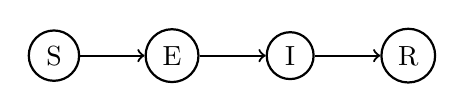
\begin{tikzpicture}[node distance={15mm}, thick, main/.style = {draw, circle}]
    \node[main] (E) {E}; 
    \node[main] (S) [left of=E] {S}; 
    \node[main] (I) [right of=E] {I}; 
    \node[main] (R) [right of=I] {R}; 
    \draw[->] (S) -- (E);
    \draw[->] (E) -- (I);
    \draw[->] (I) -- (R);
    \end{tikzpicture}
  \end{center}








\subsection{Literature Review}

Both the Hawkes and SIR models for SARS-CoV-2 have been explored in literature. Our particular interest is the comparison and connection between the two models. It is natural to compare and contrast the performance of each of these models, but analysis on their relationship and possible convergence is limited. 

~\cite{Kresin2022} discusses the relationship between the two models by mean of the reproduction number. The reproduction number notably used in the SIR model is naturally connected to the productivity constant $K$ in Hawkes, as they can both be interpreted as the expected number of infected individuals. This paper also claims that assuming an exponential triggering kernel, the intensity of the Hawkes point process is a continuous time analog to the discrete stochastic SIR model. This claim is proved in~\cite{Rizoiu2018}. Further extension on this claim is limited in literature. 

Literature regarding the use of the Hawkes process and SIR model varies in approaches and application. 










Scaling Hawkes processes to one million COVID-19 Cases
Holbrook
- Likelihood based inference requires $O(N^2)$ floating point operations for N cases
- Applies two spatiotemporal Hawkes models to the analysis of one million COVID-19 cases in the US


Opinion Market Model: stemming far-right opinion spread using positive interventions
Rizoiu
- Demonstrate the convergence of proposed estimation scheme on a synthetic dataset


Stratified epidemic model using a latent marked Hawkes process
Lamprinakou and Sandy
- Extend unstructured homogeneously mixing epidemic model to a finite population stratified by age bands
- Use latent marked Hawkes process
- Apply KDPF

Briding the COVID-19 data and the epidemiological model using the time-varying parameter SIRD model
Cakmakli and Simsek
- Extends canonical model of epidemiology SIRD model to allow for time-varying parameters for real time measurement and prediction of COVID19


A stochastic model for the early stages of highly contagious epidemics by using a state dependent point process
Casillas


Estimating COVID transmission time using Hawks point process
Schoenberg


Lecture notes for computational modelling of contagion and epidemics: a companion to the rule of contagion 
Mohler


Some statistical problems involved in foforecasting and estimating the spread of COVID19 using the Hawkes point processes and SEIR models






\section{Comparison and Connection}

Understanding the connections and differences between the Hawkes and compartmental models for COVID-19 can help deepend our understanding of the spread of the virus. This connection may enhance our ability to predict observed and latent cases, estimate pandemic-related parameters, and help understand the underlying mechanisms that drive the spread of the disease. 

Compartmental models such as SIR and SEIR are typically favoured to model COVID-19 for their physically plausible framework for the disease relative to the Hawkes model~\cite{Kresin2022}. In particular, they model the random movement of individuals between compartments and allow for the estimation of various parameters relevant to policy-makers. 

Conversely, the Hawkes model may be favoured due to its allowance of non-parametric estimation of the triggering function, spatial covariates, and ability to model how background events may trigger future events through its self-exciting properties. Additionally, this model is computationally less expensive with respect to parametric and non-parametric estimation of pandemic parameters. 



\subsection{Assumptions}
When modelling the behaviour of infectious disease, different models incorporate various assumptions to capture the dynamics of disease transmission~\cite{Kresin2022, Lamprinakou2023}. 


\subsubsection{Hawkes Model}
\begin{enumerate}
\item {\bf Self-excitement}: New infection events increase the likelihood of subsequent infections. 
\item {\bf Infinite population size}: There are an infinite number of individuals in the system.
\item {\bf Homogeneity}: Homogeneity of individuals within the population.
\item {\bf Immunity to reinfection}: Individuals are immune to reinfection for some amount of time. 
\item {\bf Epidemic trigger}: The epidemic is triggered by a set of initial infections.
\item {\bf Transition kernel is a PDF}: The transition kernel in the intensity of the process is a probability density function. 
\item {\bf Independence} The process is independent of it's time-constant parameters. 
\item {\bf Disease Transmission} Assume the transmission process of the diseasse is deterministic~\cite{Brauer2019}. 
\end{enumerate}


\subsubsection{HawkesN Model}
\begin{enumerate}
\item {\bf Self-excitement}: New infection events increase the likelihood of subsequent infections.
\item {\bf Fixed population size}: There is a finite number of individuals in the system.
\item {\bf Homogeneity}: Homogeneity of individuals within the population.
\item {\bf Immunity to reinfection}: Individuals are immune to reinfection for some amount of time. 
\item {\bf Epidemic trigger}: The epidemic is triggered by a set of initial infections. As stated by~\cite{Rizoiu2018}, it is assumed for the Maximum Likelihood estimation that the background rate is zero $\mu(t) = 0\ \forall\ t>0$. 
\item {\bf Transition kernel is a PDF}: The transition kernel in the intensity of the process is a probability density function. 
\item {\bf Independence} The process is independent of it's time-constant parameters. 
\end{enumerate}


\subsubsection{SIR Model}
\begin{enumerate}
\item {\bf Fixed population size}: There is a finite number of individuals in the system.
\item {\bf Homogeneity}: Homogeneity of individuals within the population.
\item {\bf Homogeneous mixing}: The contact of individuals is randomly distributed among the infected and susceptible populations.  
\item {\bf Short time scale:} The time scale of the SIR model is short enough that births and deaths are negligible within the system. In particular, the number of deaths from the disease is small compared to the rest of the population. 
\end{enumerate}

\subsection{Consequences}


The HawkesN is completely defined by it's parameters $\{\kappa, \theta, N \}$. Let $\mathcal{L}(\kappa, \beta, c, \theta)$ be the log-likelihood of observing a set of events $\{(m_j, t_j); j = 1, \ldots, n\}$ in a non-homogeneous Poisson process with rate $\lambda^H(t)$~\cite{Rizoiu2018}. Note that we assume the background rate to be zero, $\mu(t) = 0 \ \forall\ t>0$. Equivalently, we that apart from the first, each event is a result of the initial event. Then,
\[
\mathcal{L}(\kappa, \beta, c, \theta) = \sum_{j=1}^n \log (\lambda^H (t_j^-)) - \int_0^{t_n} \lambda^H (\tau) d \tau
\]


It is claimed that most compartmental models can be represented using a renewal equation~\cite{Kresin2022}. This naturally bridges a connection be the two models as both the reproduction number in the renewal equation and productivity constant $K$ in Hawkes can both be interpreted as the expected number of direct transmission per infected individual.


\cite{Rizoiu2018} further discusses connections between the two frameworks. They claim that the rate of events in an extended Hawkes model is identical to the rate of new infection in the SIR model. 
\\

\begin{theorem}\label{thrm:SIR}
Suppose the new infections in a stochastic SIR process of parameters $\{\beta, \gamma, N\}$ follow a point process of intensity $\lambda^I(t)$. Suppose also that the events in a HawkesN process with parameters $\{\mu, K, \theta, N\}$ have intensity $\lambda^H (t)$ with an exponential kernel such that,
\[
\phi(\tau) =  \theta e^{-\theta \tau}, \hspace{5mm} \text{and} 
\]
Let $\tau^R$ = $\{\tau_1^R, \tau_2^R, \ldots \}$ be the set of the times to recovery of the infected individuals in the SIR process. the expectation of $\lambda^I (t)$ over $\tau^R$ is equal $\lambda^H (t)$:
\[
\mathbb{E}_{\tau^R} [ \lambda^I (t)] = \lambda^H (t)\]

when $\mu = 0$, $\beta = K \theta$, and $\gamma = \theta$~\cite{Rizoiu2018}. c
\end{theorem}



\begin{proof} Recall that $C_t$ denotes the infection process, and $R_t$ denotes the recovery process. First, we write these using the sum of indicators functions. We find that
\begin{align*}
S_t &= N - C_t = N - \sum_{j\geq 1} \mathbbm{1} (t_j^I < t) \\
I_t &= C_t - R_t = \sum_{j\geq 1} \mathbbm{1} (t_j^I < t, t_j^R > t) = \sum_{t_j^I < t} \mathbbm{1} (t_j^I + {\tau^R}_j > t). 
\end{align*} 
 
Consider the point process consisting of only the infection events $\{t_j^I\}$. The event rate in this process is obtained by marginalizing out times of recovery. 
\begin{align*}
\mathbb{E}_\omega [ \lambda^I (t)] 
&= \mathbb{E}_{\tau^R} \Big [\beta \frac{S_t}{N} \sum_{t_j^I < t} \mathbbm{1} (t_j^I + {\tau^R}_j > t) \Big ]\\ 
&= \sum_{t_j^I < t} \mathbb{E}_{\tau^R} \Big [\beta \frac{S_t}{N}  \mathbbm{1} (t_j^I + {\tau^R}_j > t) \Big ]\\
&= \sum_{t_j^I < t}\int_0^\infty \beta \frac{S_t}{N}  \mathbbm{1} (t_j^I + \zeta > t) r_{\tau^R}(\zeta) d\zeta \\
&= \sum_{t_j^I < t} \beta \frac{S_t}{N} \int_{t - t_j^I}^\infty r_{\tau^R}(\zeta) d\zeta \\
&= \sum_{t_j^I < t} \beta \frac{S_t}{N} \int_{t - t_j^I}^\infty r_{\tau^R}(\zeta) d\zeta
\end{align*}
 
where $r_{\tau^R}(\zeta)$ is the exponential probability distribution function for the time of recovery. Since $S_t = N - C_t$, we get
\[
\mathbb{E}_{\tau^R} [ \lambda^I (t)] = \Big (1 - \frac{C_t}{N} \Big ) \sum_{t_j^I < t}  \beta e^{- \gamma (t - t_j^I)}
\] 
 
 
 
\end{proof}





%--------

%TODO: 
%- Hawkes likelihood
%- appendix C.3 equivalence to stochastic SIR


\subsubsection{Exploration of Triggering Kernel}

\cite{Rizoiu2018} shows equivalence in expectation between the intensities of the stochastic SIR and HawkesN models. We want to explore if any other choices in the triggering kernel $\phi(\cdot )$ of the HawkesN process yields more connection between the Hawkes model and other stochastic representations of other compartmental models. 

First recall the SEIR model, in definition~\ref{SEIR}. Consider the stochastic representation of this  model with random variables $S_t$, $E_t$, $I_t$, and $R_t$ associated with their respective compartments. Suppose the new infections in this stochastic SEIR process of intensity $\lambda^I(t)$, as in definition~\ref{stochastic-SIR}.

Recall the $C_t$ is the counting process associated with the infection process and $R_t$ is the counting process associated with the recovery process. Then $C_t$ is the cumulative number of occurred infections, including individuals that may still be infectious. 

By definition of the SEIR model, we naturally have that $N = S_t + E_t + I_t + R_t$. Encorporating the cumulative case count $C_t$, we also get

\[
S_t = N - C_t, \hspace* {5mm}
I = C_t - R_t  - E_t
\]

Equivalently to the above, we have that

\[
C_t = N - S_t
\]

% We define the intensity of a stochastic compartmental model, in this case the SEIR model, as the rate of change of individuals moving into the infected compartment. Equivalently, this is the rate of change of $C_t$. That is, 

% \begin{align*}
%   \lambda^I(t) &= \frac{dC_t}{dt} \\
%   &= \frac{d (N - S_t - E_t)}{dt} \\
%   &= - \frac{d(S_t + E_t)}{dt} \\
%   &= - \Big ( \frac{dS_t}{dt} + \frac{dE_t}{dt} \Big ) \\
%   &= aE
% \end{align*}

%maybe definition of incubation period is not accurate?
%cite how we know incubation times are 


%TODO work on notation and flow here
Consider the time period $(t_j^E, t_j^I)$, the time that it takes for an individual to become infected after being exposed to a disease. Define the \textit{time to infection from exposed}, $\tau_j^{I} = t_j^I - t_j^E$, to be the time in which individual $j$ is exposed to the disease before becoming infected. We assume that the these times are exponentially distributed with parameter $a$, and mean wait time $1/a$. Let $r_\tau^{I}(\zeta)$ be the probability distribution function for $\tau^I$. 
%theta_I = a


% this needs more explanation i think
% I think the distirbution of the wait times would only be a convolution if there were intermittend steps/compartments within the E compartment. Since S is not consideed in the incubation times, would it still be a convolution?

% \begin{theorem}[TODO]
%   %TODO

%   Let $\omega = \{\omega_1, \omega_2, \ldots\}$ be the set of incubation times for each individual in the SEIR model. 
% \end{theorem}

% \begin{proof}
  

% \begin{align}
%   \mathbb{E} [\lambda^I (t)] &= \mathbb{E}_\omega [a E_t] \\
%   &= \mathbb{E}_\omega [a \sum_{j\geq 1} \mathbbm{1}(t_j^E < t, t_j^I > t)] \\ 
%   &= \mathbb{E}_\omega [a \sum_{j\geq 1} \mathbbm{1}(t_j^I - \omega_j^{(EI)}  < t)] \\
%   &= \sum_{j\geq 1} \int_0^{\infty} a \mathbbm{1}(t_j^I - \zeta < t) r_\tau(\zeta) d \zeta \\
%   &= \sum_{j\geq 1} a \int_{t_j^I - t}^{\infty} r_\omega(\zeta) d\zeta \\
%  % &= a \sum_{j\geq 1} e^{-\gamma (t_j^I - t)}
% \end{align}


% \end{proof}



Now, consider the stoachastic representation of the SEIR model. We aim to connect the intensity of this model to the intesity of the HawkesN process. Note the added `exposed' comparment in the SEIR model in comparison to the more simple SIR model. Individuals associated with this compartment are classified as infected but not \textit{infectious}. In other words, these individuals are carrying and potentially spreading the disease, despite not belonging to the infected compartment.

By definition, the relevant intensity associated with the stochastic representation of the SEIR model is the rate at which individuals in the population become inftenced– or the rate at which indivuals enter the $E$ compartment. Equivalently, the intensity of the stoachastic SEIR model is precisely the rate of change of the cumulative case counts. Note in the following that it continues to hold that $C_t = N - S_t$. 

\begin{equation}
  \lambda^{E}(t) = \frac{d C_t}{dt} =  -\frac{dS_t}{dt} = \beta \frac{IS}{N}
\end{equation}

We additionally aim to write $I_t$ as the sum of indicators. 

\begin{align*}
  I_t &= C_t - R_t - E_t  \\
  &= \sum_{j \geq 1} \mathbbm{1} (t_j^I < t, t_j^R > t) \\
  &=  \sum_{t_j^I < t} \mathbbm{1} (t_j^I + \tau_j^R > t) \\
  &=  \sum_{t_j^E + \tau_j^I < t} \mathbbm{1} (t_j^E + \tau_j^I + \tau_j^R > t) 
\end{align*}



\begin{theorem}\label{thrm:SEIR}
  Suppose the new infections in a stoachastic SEIR process of parameters $\{\beta, a, \gamma, N\}$ follow a point process of intensity $\lambda^E(t)$. Suppose also that the vents in a HawkesN process with parameters $\{\mu, K, \theta, N\}$ have intensity $lambda^H(t)$ with an exponential kernal such that,
  \[
  \phi(\tau) = \theta e^{-\theta \tau}, \hspace{5mm} \text{and,} \theta > a.
  \]

  Let $\tau_I = \{\tau_1^I, \tau_2^I, \ldots\}$ and $\tau_R = \{\tau_1^R, \tau_2^R, \ldots\}$ be the set of times to infectious from exposed and times to recover from infectious respectively. The expectation of $\lambda^E(t)$ over the wait times is equal to $\lambda^H(t)$:

  %TODO - be careful between infected and infectious --> go back up and clarify

  \[
\mathbb{E}[\lambda^E(t)] = \lambda^H(t)
  \]
  when $\mu=0$, $\beta=\frac{\theta - a}{a} \theta$, and $\gamma = \theta$. 
\end{theorem}

\begin{proof}
  
  

% \begin{align*}
%   \lambda^{E}(t) &= \mathbb{E}_{\tau^R} \Big [ \beta \frac{S_t}{N} I_t  \Big ] \\
%   &= \mathbb{E}_{\tau^R} \Big [ \beta \frac{S_t}{N}  \sum_{t_j^I < t} \mathbbm{1} (t_j^I + \tau_j^R > t)  \Big ] \\
%   &=  \mathbb{E}_{\tau^I} \mathbb{E}_{\tau^R} \Big [ \beta \frac{S_t}{N}  \sum_{t_j^I < t} \mathbbm{1} (t_j^E + \tau_j^I + \tau_j^R > t)  \Big ] \\
%   &=  \sum_{t_j^I < t} \mathbb{E}_{\tau^I} \mathbb{E}_{\tau^R} \Big [ \beta \frac{S_t}{N} \mathbbm{1} (t_j^E + \tau_j^I + \tau_j^R > t)  \Big ] \\
%   &=  \sum_{t_j^I < t} \int_0^\infty \int_0^\infty \beta \frac{S_t}{N}  \mathbbm{1} (t_j^E + \zeta^I + \zeta^R > t)\ r_{\tau_R}(\zeta^R) r_{\tau_I}(\zeta^I) d\zeta^R\ d\zeta^I \\
%   &=  \sum_{t_j^I < t} \beta \frac{S_t}{N} \int_{0}^\infty \int_{t-t_j^E-\zeta^I}^\infty \ r_{\tau_R}(\zeta^R) r_{\tau_I}(\zeta^I) d\zeta^R\ d\zeta^I \\
%   &=  \sum_{t_j^I < t} \beta \frac{S_t}{N} \int_{0}^\infty  e^{-\theta_R (t - t_j^E - \zeta^I)} r_{\tau_I}(\zeta^I) d\zeta^R\ d\zeta^I \\
%   &=  \sum_{t_j^I < t} \beta \frac{S_t}{N} \int_{0}^\infty  e^{-\theta_R (t - t_j^E - \zeta^I)} \theta_I e^{-\theta_I \zeta^I} d\zeta^R\ d\zeta^I \\
%   &=  \sum_{t_j^I < t} \beta \frac{S_t}{N} e^{-\theta_R (t - t_j^E)} \int_{0}^\infty   \theta_I e^{-(\theta_I - \theta_R) \zeta^I} d\zeta^R\ d\zeta^I \\
%   &=  \sum_{t_j^I < t} \beta \frac{S_t}{N} e^{-\theta_R (t - t_j^E)} \frac{\theta_I}{\theta_I - \theta_R} \\
%   &=  \Big ( 1 - \frac{C_t}{N} \Big )  \sum_{t_j^I < t} \frac{\theta_I}{\theta_I - \theta_R} \beta e^{-\theta_R (t - t_j^E)}  \\
% \end{align*}



% - clean up what we're summing over
% - I can't change the integral with the sum --> this is where the convolution comes from

\begin{align*}
  \lambda^{E}(t) &= \mathbb{E}_{\tau^R} \Big [ \beta \frac{S_t}{N} I_t  \Big ] \\
  &= \mathbb{E}_{\tau^R} \Big [ \beta \frac{S_t}{N}  \sum_{t_j^I < t} \mathbbm{1} (t_j^I + \tau_j^R > t)  \Big ] \\
  &=  \mathbb{E}_{\tau^I} \mathbb{E}_{\tau^R} \Big [ \beta \frac{S_t}{N}  \sum_{t_j^I < t} \mathbbm{1} (t_j^E + \tau_j^I + \tau_j^R > t)  \Big ] \\
  &= \beta \frac{S_t}{N} \mathbb{E}_{\tau^I} \Big [ \int_0^\infty  \sum_{t_j^E + \tau_j^I < t} \mathbbm{1} (t_j^E + \tau_j^I + \zeta^R > t) r_{\tau^R}(\zeta^R) d \zeta^R  \Big ] \\
  &= \beta \frac{S_t}{N} \mathbb{E}_{\tau^I}  \Big [ \sum_{t_j^E + \tau_j^I < t} \int_0^\infty  \mathbbm{1} (t_j^E + \tau_j^I + \zeta^R > t) r_{\tau^R}(\zeta^R) d \zeta^R  \Big ] \\
  &= \beta \frac{S_t}{N} \mathbb{E}_{\tau^I}  \Big [ \sum_{t_j^E + \tau_j^I < t} \int_{t - t_j^E - \tau_j^I}^\infty r_{\tau^R}(\zeta^R) d \zeta^R  \Big ] \\
  &= \beta \frac{S_t}{N} \mathbb{E}_{\tau^I}  \Big [ \sum_{t_j^E + \tau_j^I < t} e^{-a(t-t_j^E-\tau_j^I)}  \Big ] \\
  &= \beta \frac{S_t}{N} \int_0^\infty \Big (  \sum_{t_j^E + \zeta^I < t} e^{-a(t-t_j^E-\zeta^I)}  \Big ) r_{\tau^I} (\zeta^I) d\zeta^I \\
  &= \beta \frac{S_t}{N} \int_0^\infty \Big (  \sum_{t_j^E + \zeta^I < t} e^{-a(t-t_j^E-\zeta^I)}  \Big ) \theta e^{-\theta \zeta^I} d\zeta^I \\
  &= \beta \frac{S_t}{N}  \theta \int_0^\infty e^{\zeta^I(a-\theta)} \sum_{t_j^E + \zeta^I < t} e^{-a(t-t_j^E)}   d \zeta^I \\
  &= \beta \frac{S_t}{N}  \theta \int_0^\infty e^{\zeta^I(a-\theta)} \sum_{j \geq 1} \mathbbm{1} (t_j^E + \zeta^I < t) e^{-a(t-t_j^E)}   d \zeta^I \\
  &= \beta \frac{S_t}{N}  \theta \sum_{j \geq 1} \int_0^\infty e^{\zeta^I(a-\theta)}  \mathbbm{1} (t_j^E + \zeta^I < t) e^{-a(t-t_j^E)}   d \zeta^I \\
  &= \beta \frac{S_t}{N}  \theta \sum_{j \geq 1}  e^{-a(t-t_j^E)}  \int_0^{t-t_j^E} e^{\zeta^I(a-\theta)}  d  \zeta^I \\
  &= \beta \frac{S_t}{N}  \theta \sum_{j \geq 1}  e^{-a(t-t_j^E)}  \frac{e^{(t-t_j^E)(a - \theta)} - 1}{a - \theta}\\
  &= \beta  \frac{S_t}{N} \frac{\theta }{a - \theta } \sum_{j \geq 1}e^{-a(t-t_j^E)}  (e^{(t-t_j^E)(a - \theta)} - 1) \\
\end{align*}

since it is assumed that $\theta - a > 0$.

\end{proof}


%TODO unfinished



%We aim to write $S_t$ and $I_t$

\section{Implementation}

A Monte Carlo simulation with 20 repetitions are run, each with population size $N = 1300$, and theoretical parameters $I = 300$, $\gamma = 0.2$, and $\beta = 1$. These are adapted from code provided by \citep{Rizoiu2018}.  It is important to note that the code is modified with the assumption that the total population size $N$ is known. Hence, any estimation of $N$ is omitted from the adapted code. The code produces synthetic data suitable for the models of interest. The SIR data is represented with a set of unique timepoints. Each timepoint $t$ is associated with a number representing each compartment, $S_t$, $I_t$, $R_t$, and $C_t$, where $C_t = I_t + R_t$ is infection process. 
 
The HawkesN data is transformed using the SIR data to be represented by the timepoints associated with each infection event. Moreover, by Theorem~\ref{thrm:SIR}, the estimated parameters from the HawkesN model can be transformed to analogous SIR results using the following:
\[
\gamma = \theta, \hspace{10mm}
\beta = \kappa \theta
\]

We aim to estimate $\beta$ and $\gamma$ in the SIR model, as well as $\kappa$ and $\theta$ in the HawkesN. We plot the likelihood for each parameter. 




\section{Results}

Figures~\ref{fig:SIR-ll} and~\ref{fig:HawkesN-ll} reflect the negative log-likelihood of the parameters associated with the SIR model and HawkesN model respectively. Figure~\ref{fig:contour} shows a contour plot for each model between each pairs of parameters. 








\begin{figure}
\centering
\begin{subfigure}{.5\textwidth}
  \centering
  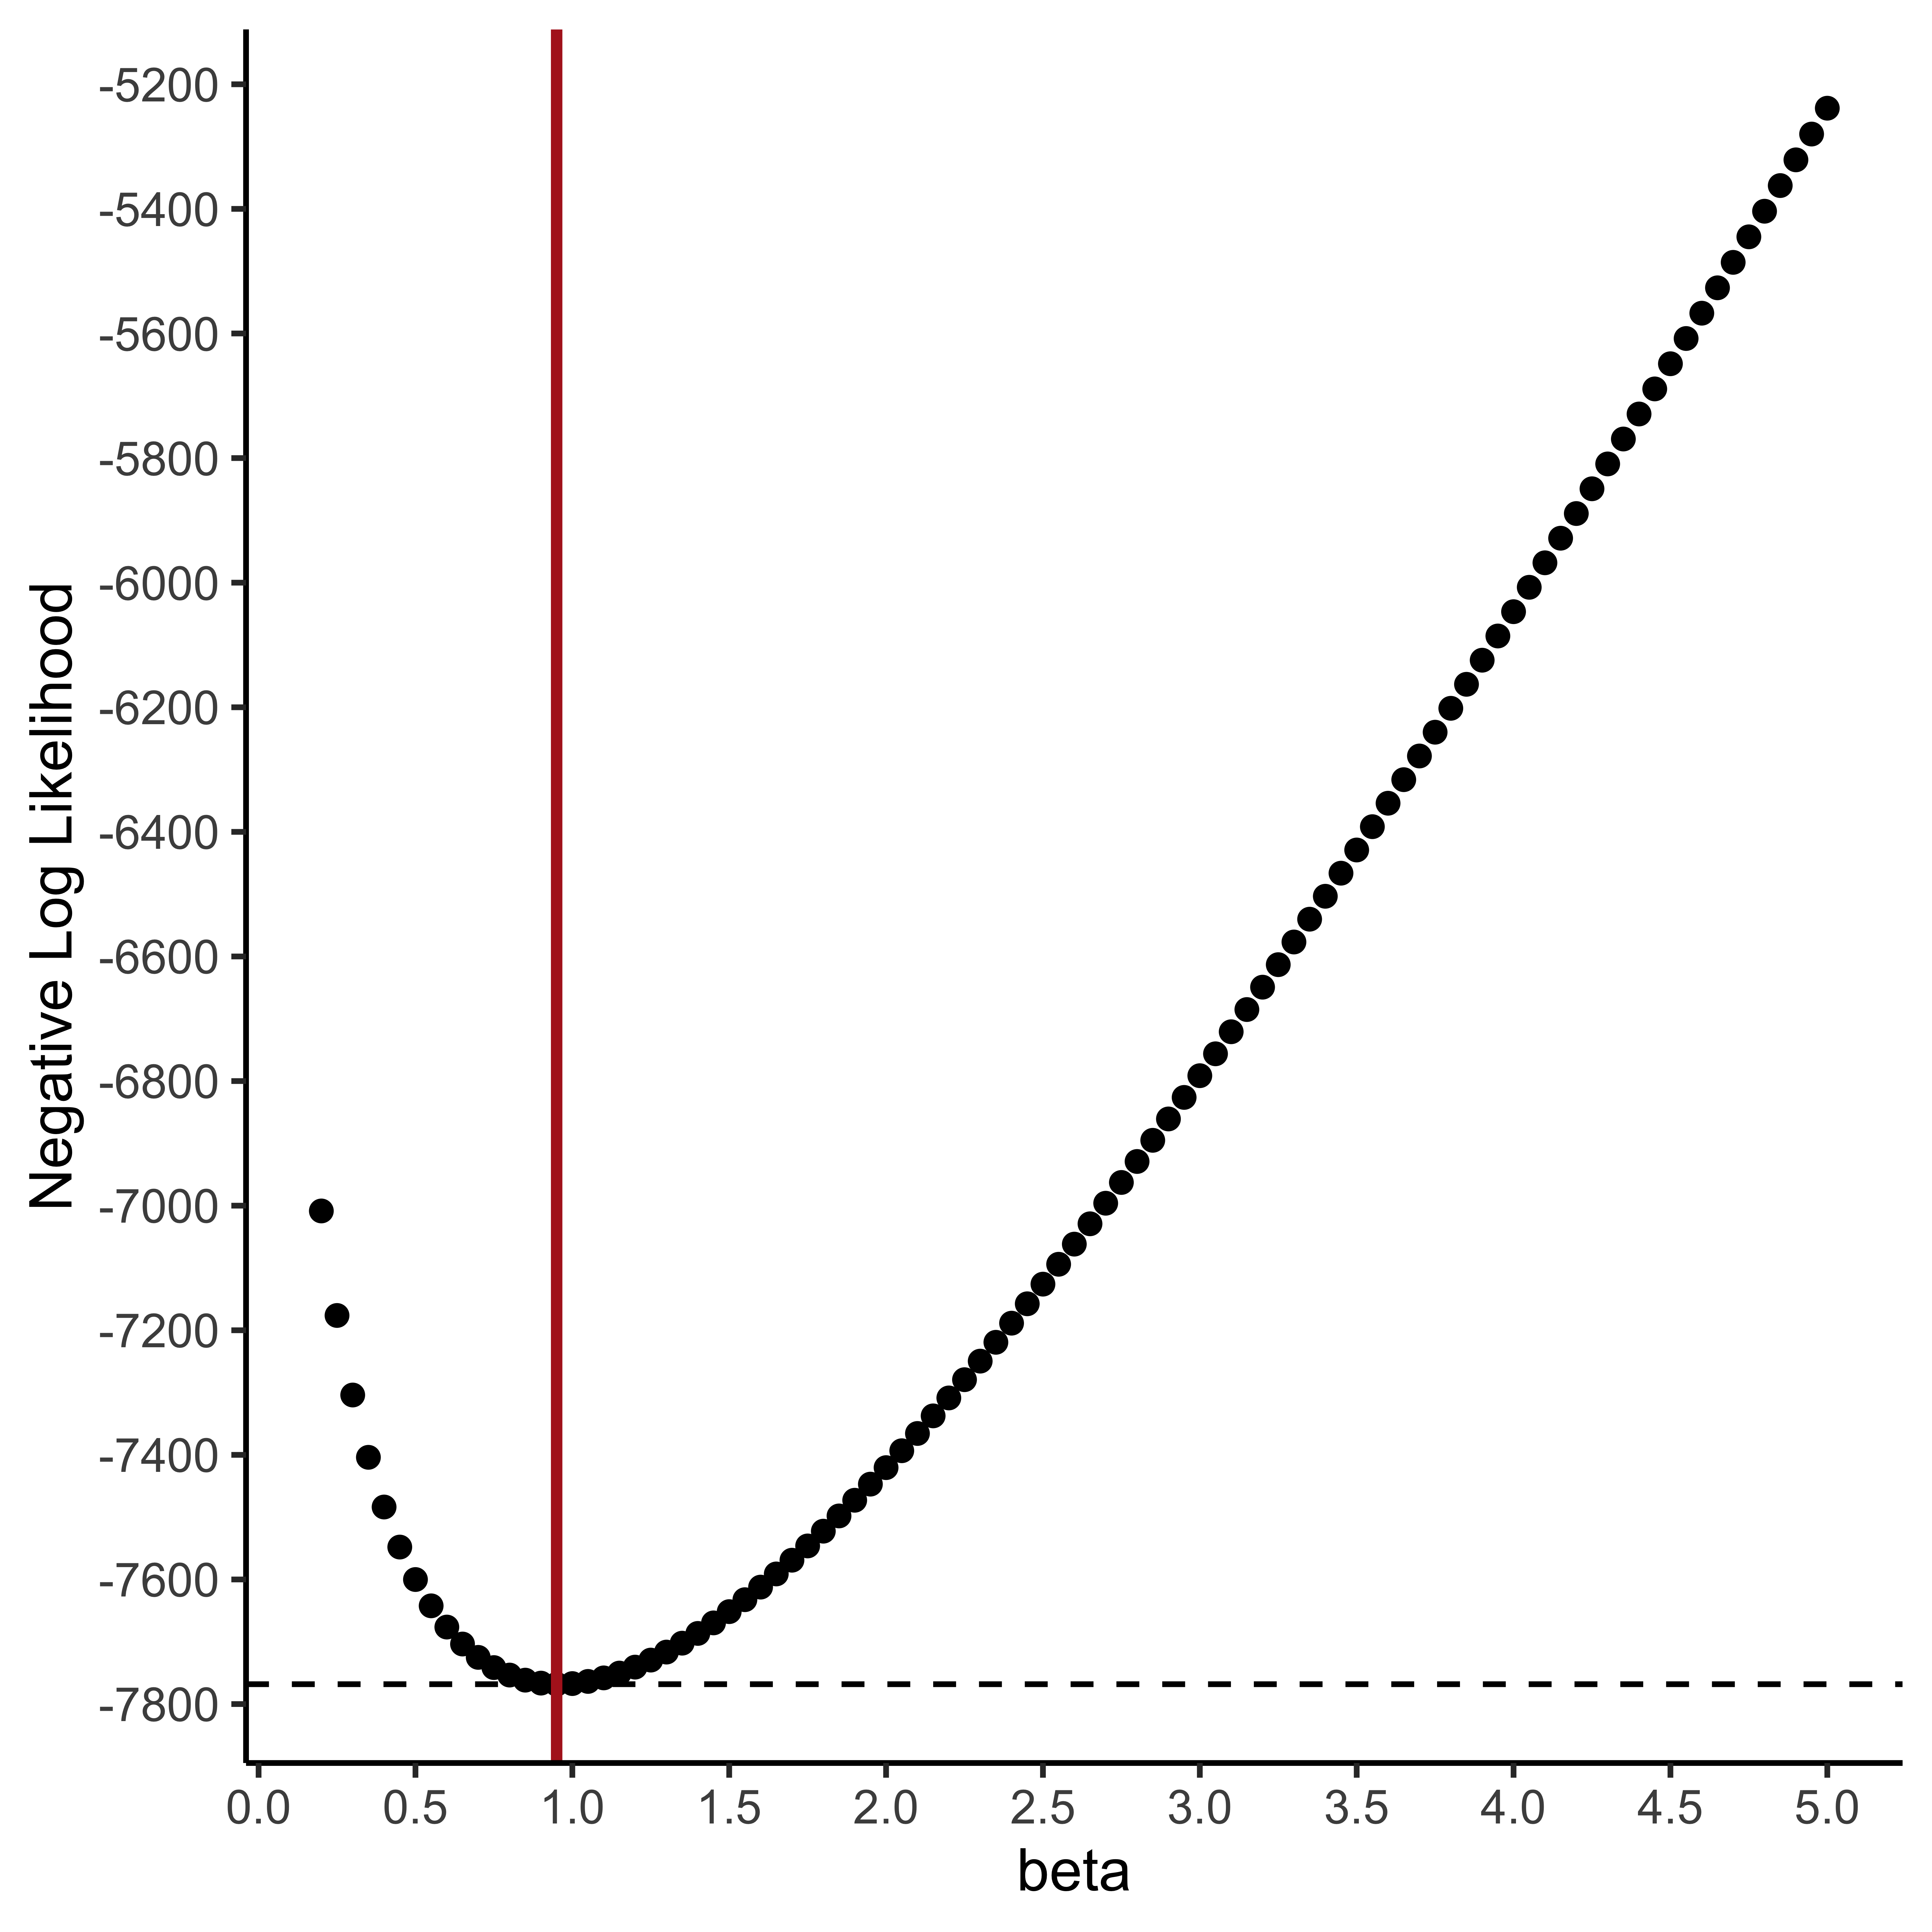
\includegraphics[width=0.9\linewidth]{../figures/SIR_neg-log-likelihood-plot_beta.png}
  \caption{$\beta$}
\end{subfigure}%
\begin{subfigure}{.5\textwidth}
  \centering
  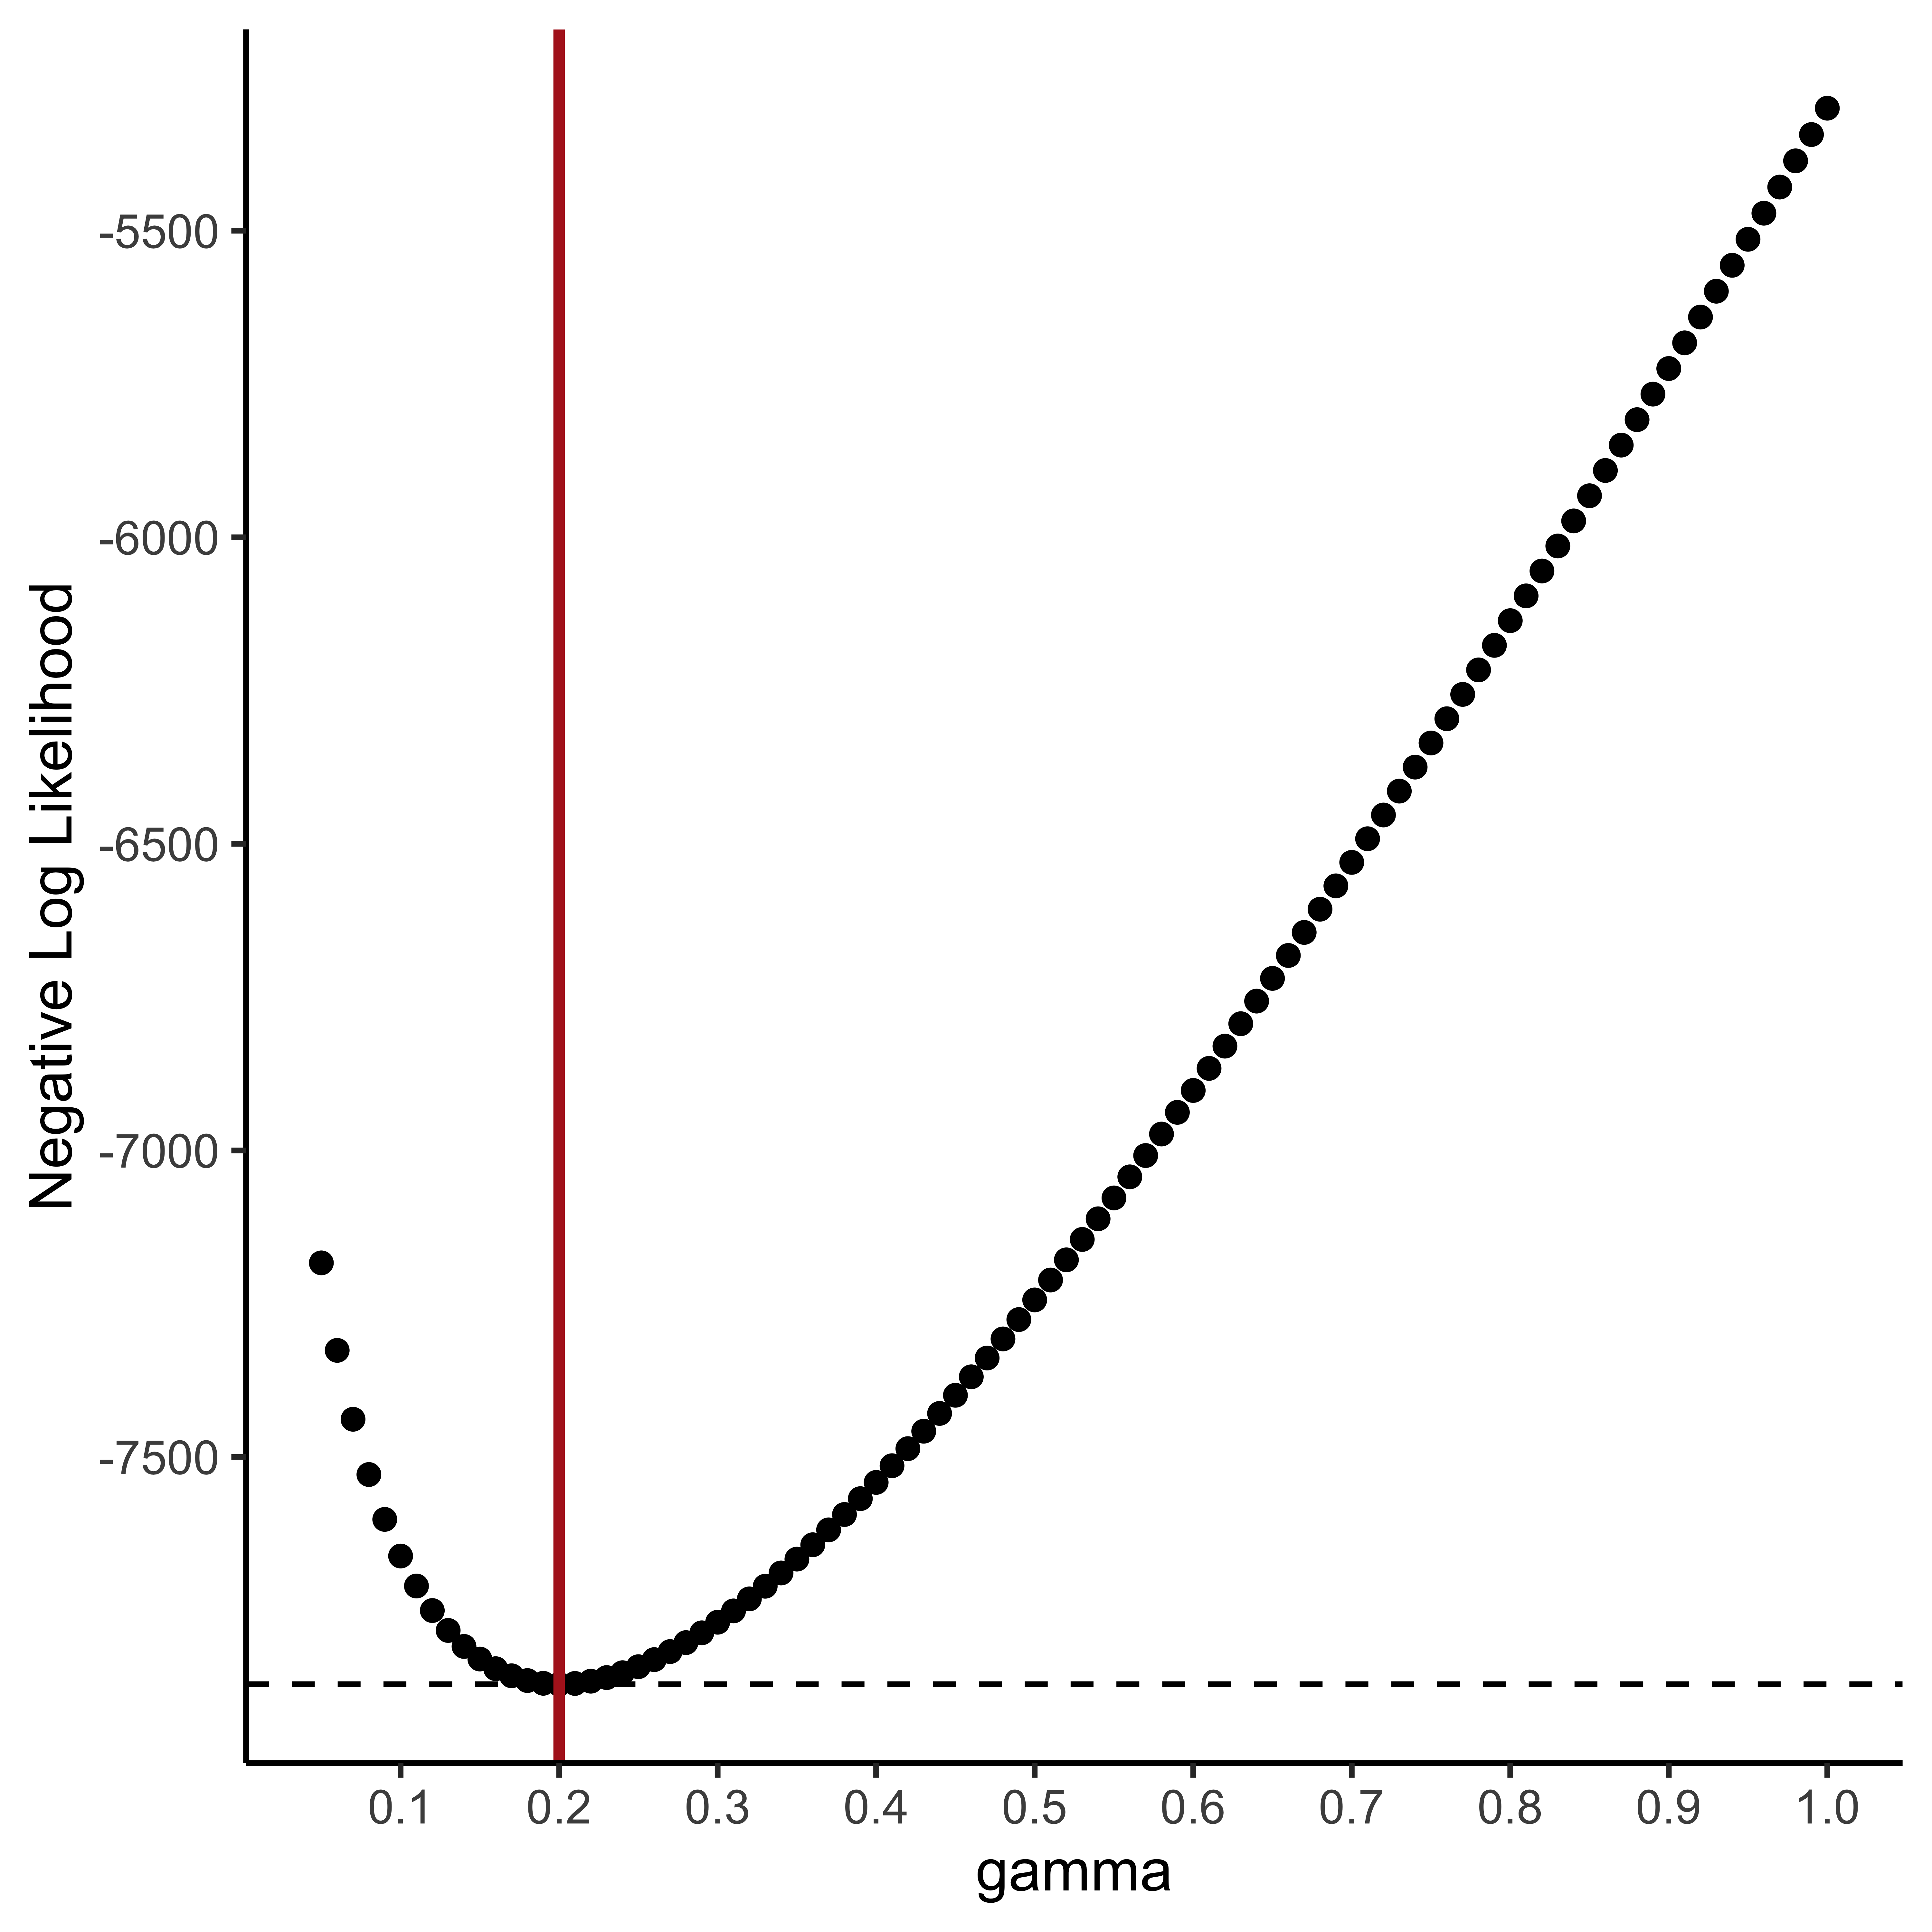
\includegraphics[width=0.9\linewidth]{../figures/SIR_neg-log-likelihood-plot_gamma.png}
  \caption{$\gamma$}
\end{subfigure}
\caption{Negative log-likelihood plot of parameters for HawkesN model. }\label{fig:SIR-ll}
\end{figure}



\begin{figure}
\centering
\begin{subfigure}{.5\textwidth}
  \centering
  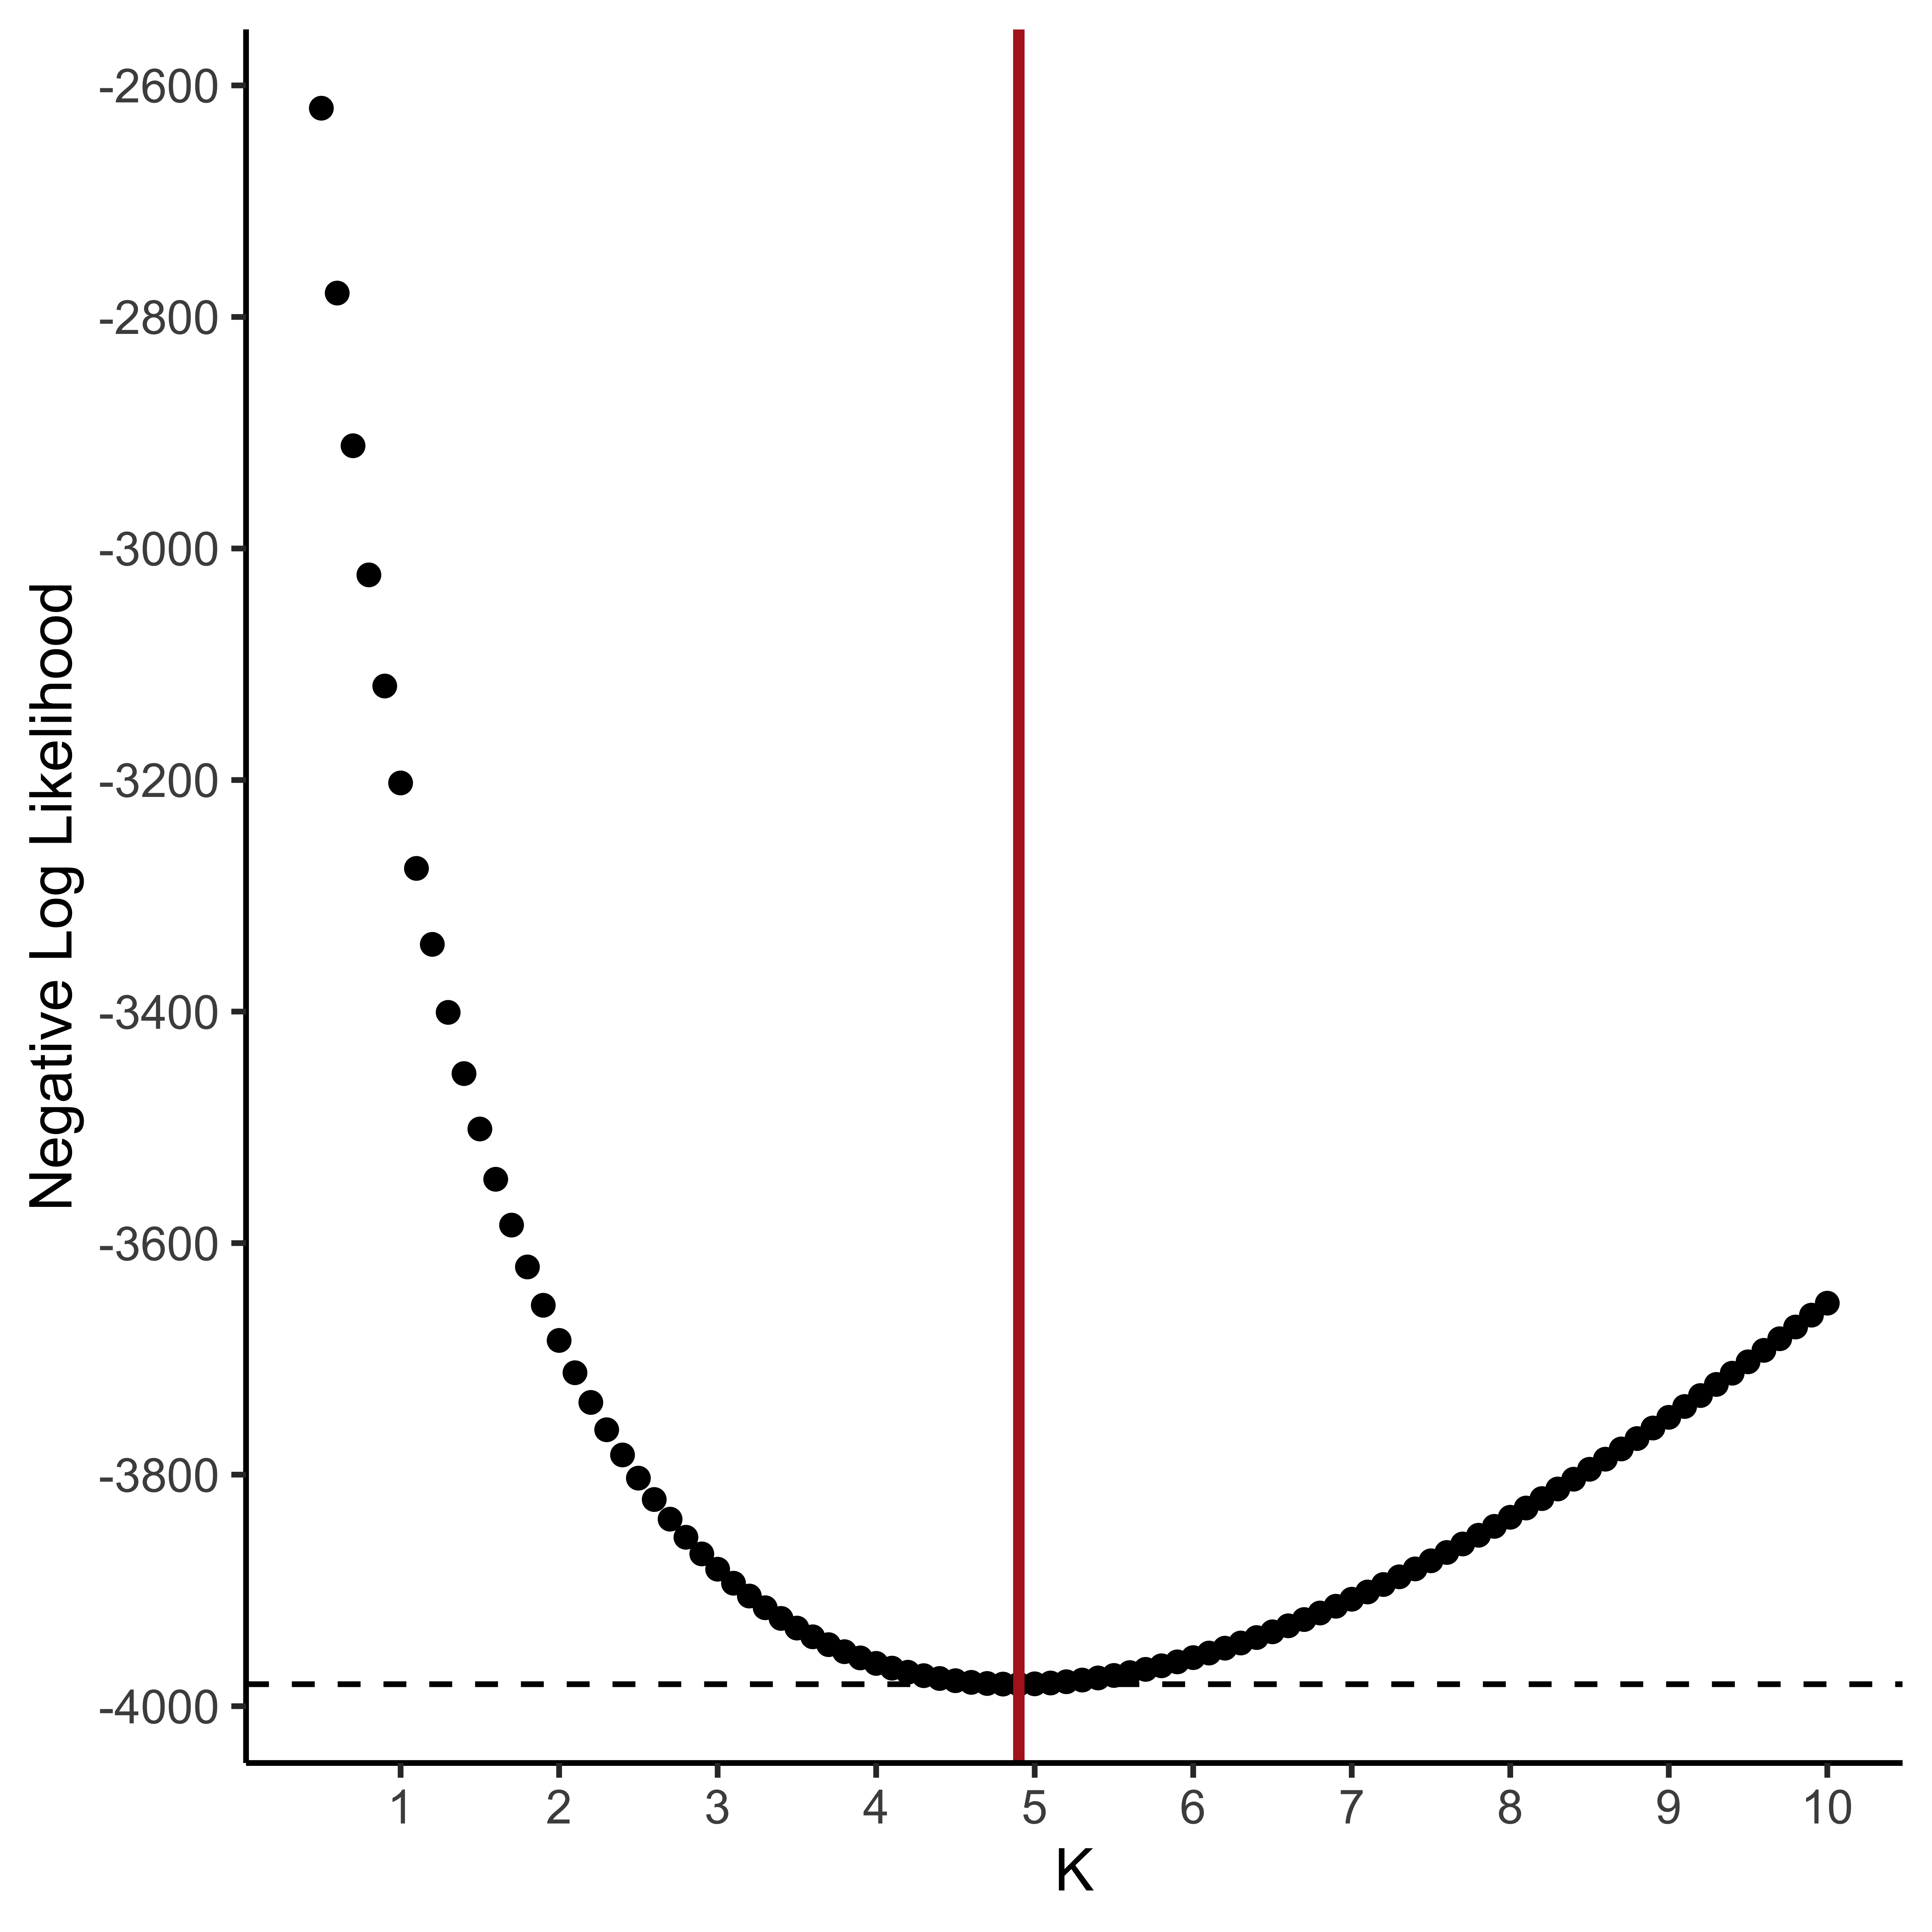
\includegraphics[width=0.9\linewidth]{../figures/HawkesN_neg-log-likelihood-plot_K.png}
  \caption{$K$}
\end{subfigure}%
\begin{subfigure}{.5\textwidth}
  \centering
  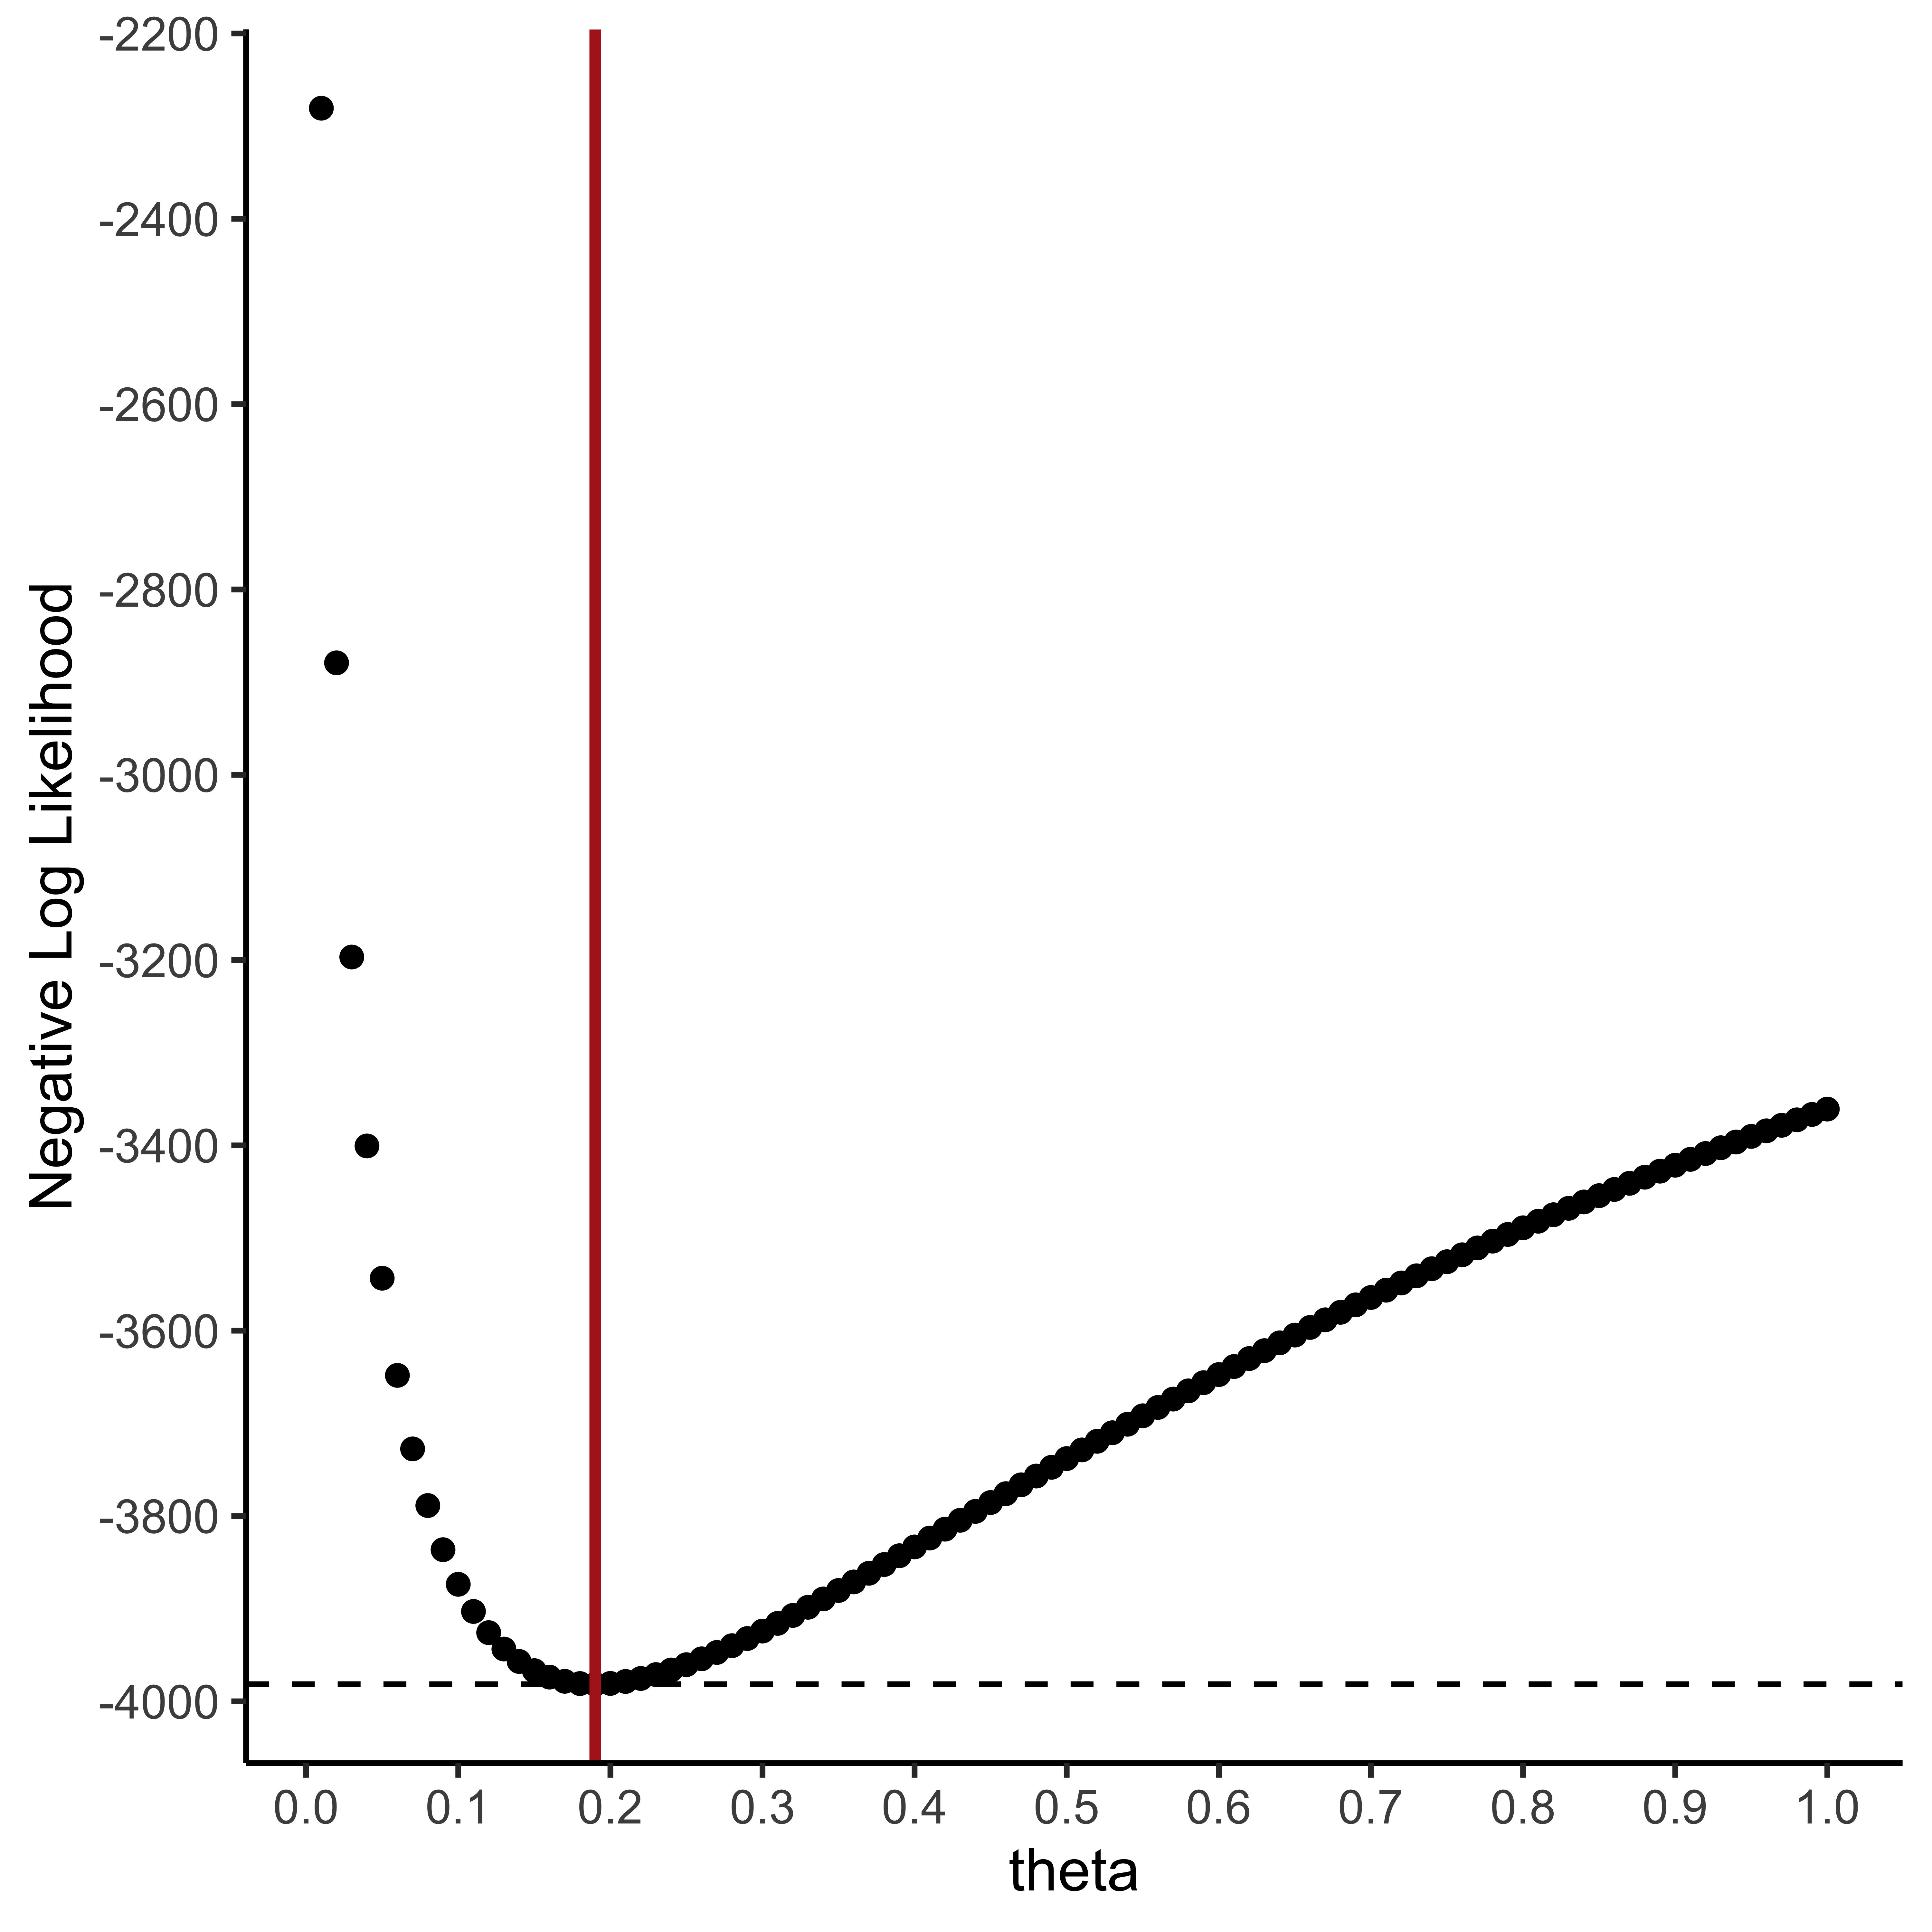
\includegraphics[width=0.9\linewidth]{../figures/HawkesN_neg-log-likelihood-plot_theta.png}
  \caption{$\theta$}
\end{subfigure}
\caption{Negative log-likelihood plot of parameters for HawkesN model. }\label{fig:HawkesN-ll}
\end{figure}


\begin{figure}
\centering
\begin{subfigure}{.5\textwidth}
  \centering
  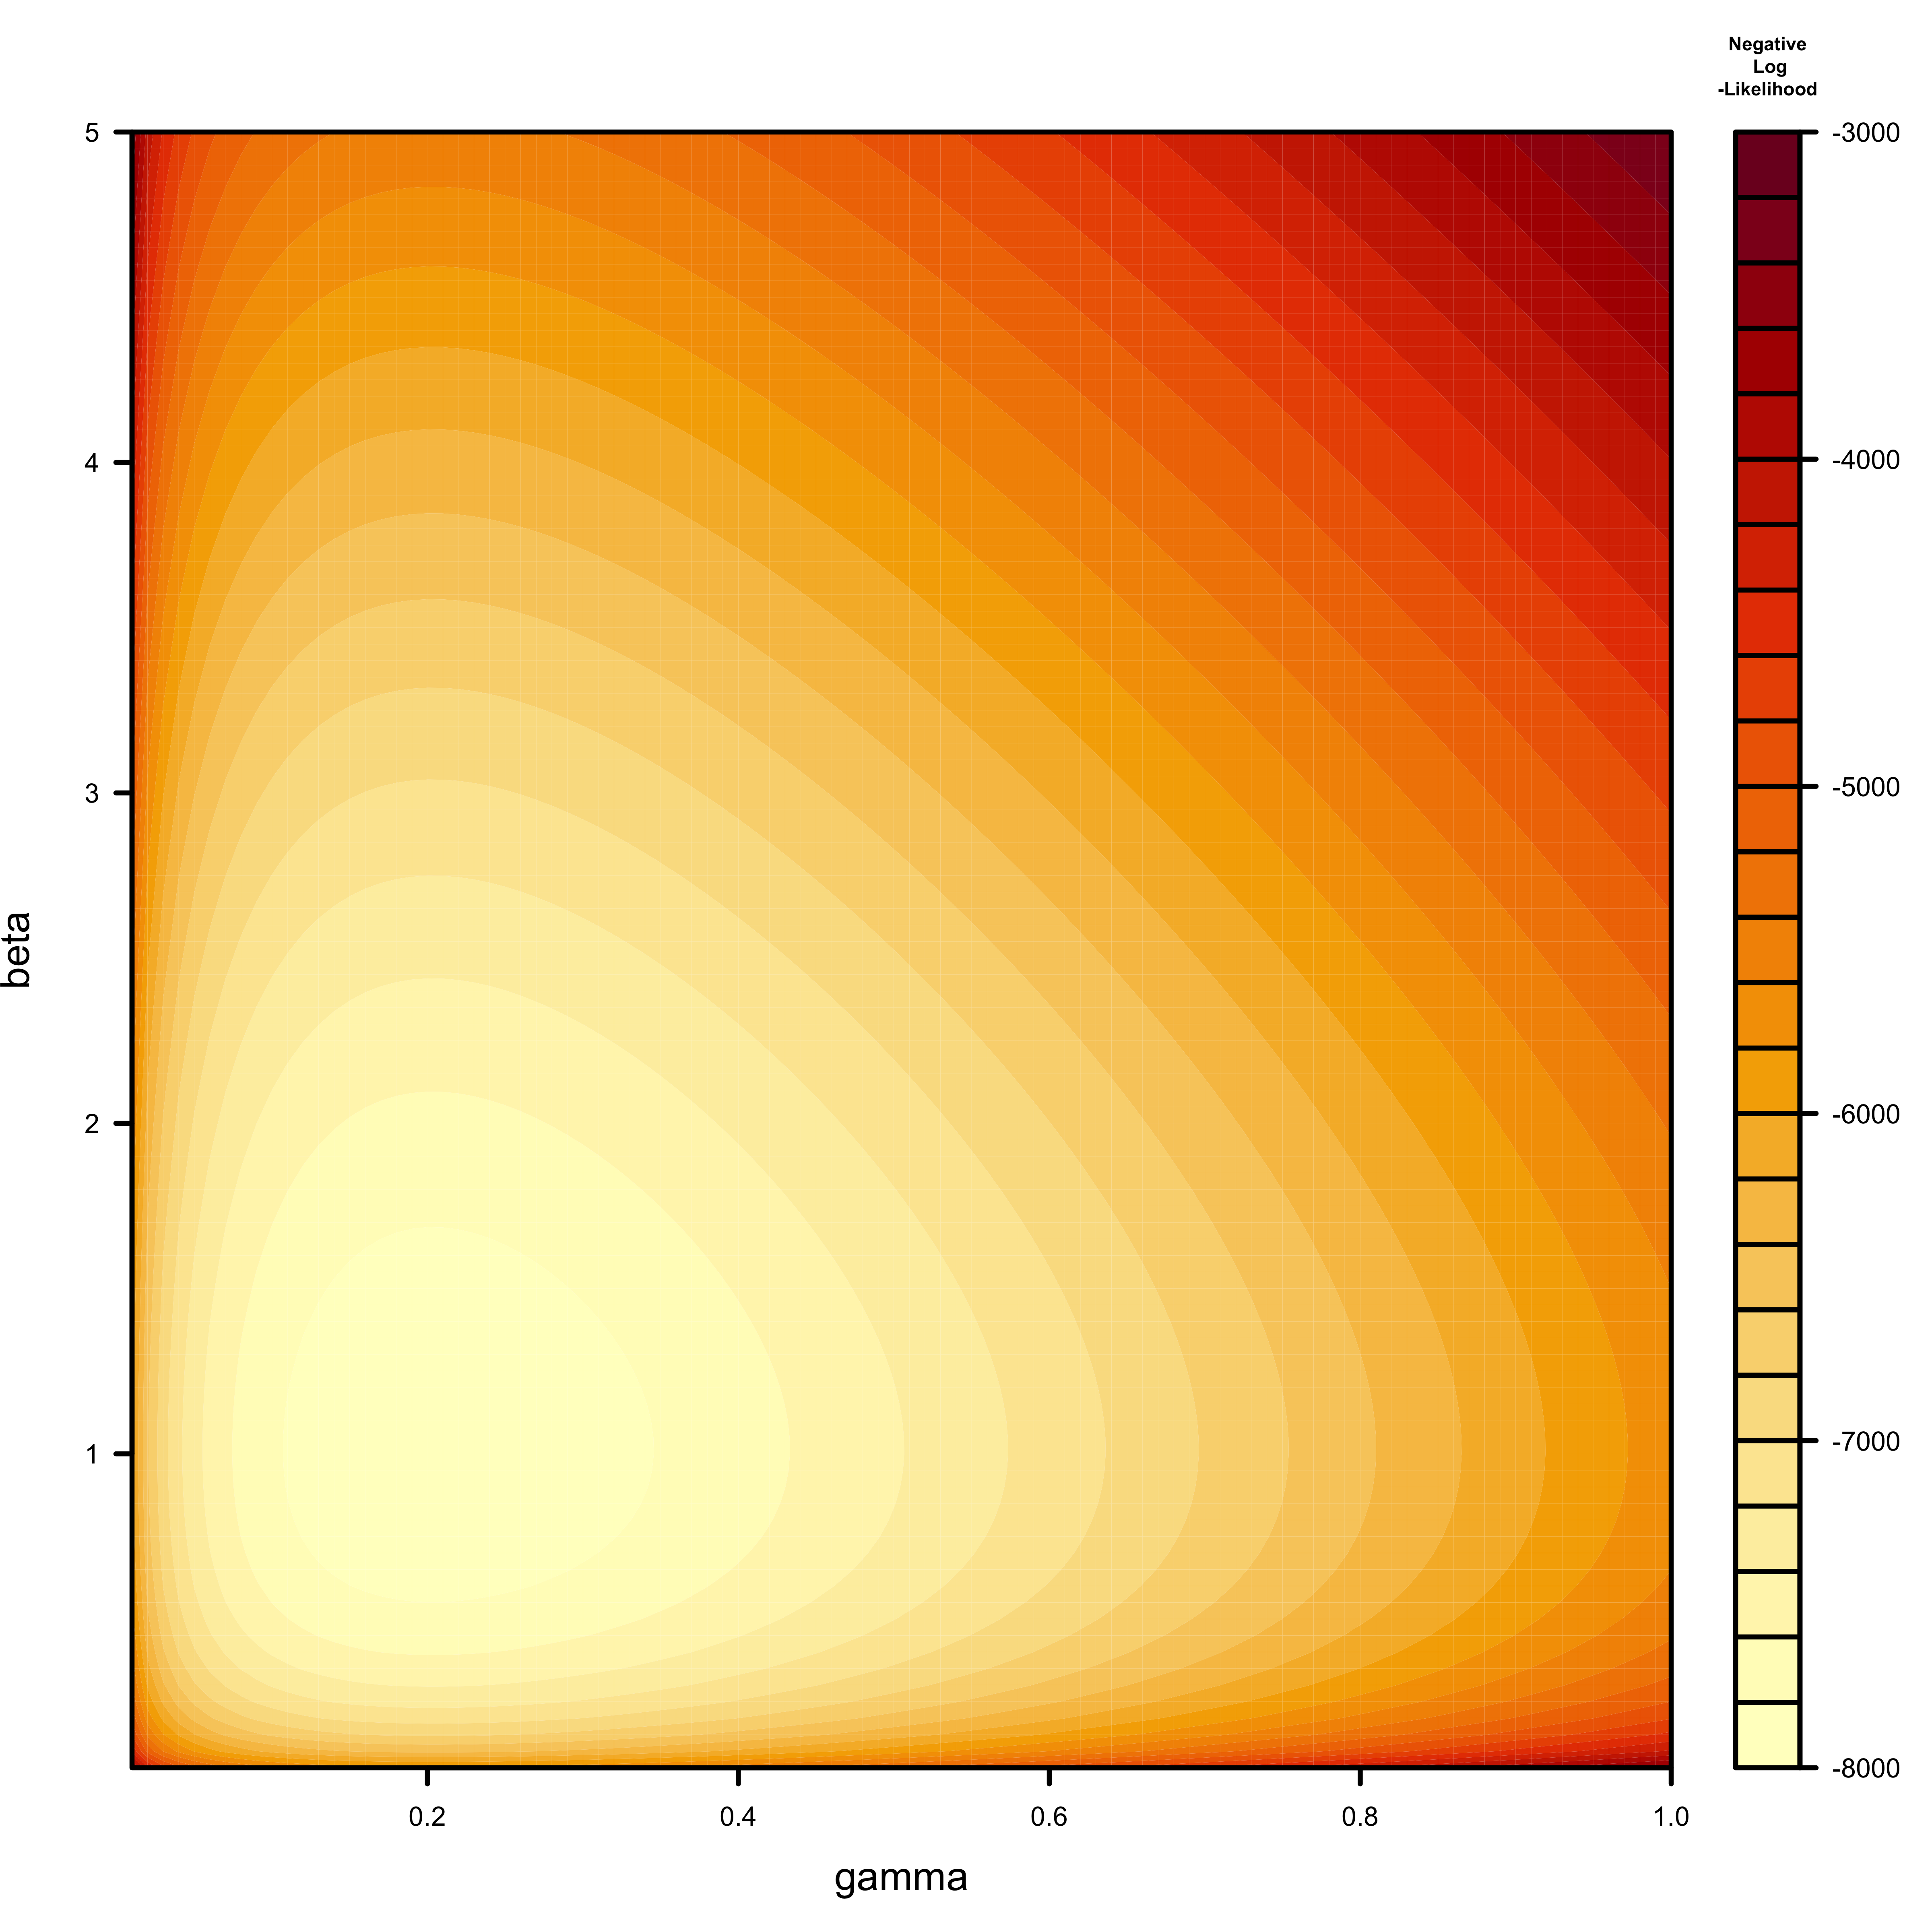
\includegraphics[width=1\linewidth]{../figures/SIR_contour-plot_gamma_beta.png}
  \caption{SIR}
\end{subfigure}%
\begin{subfigure}{.5\textwidth}
  \centering
  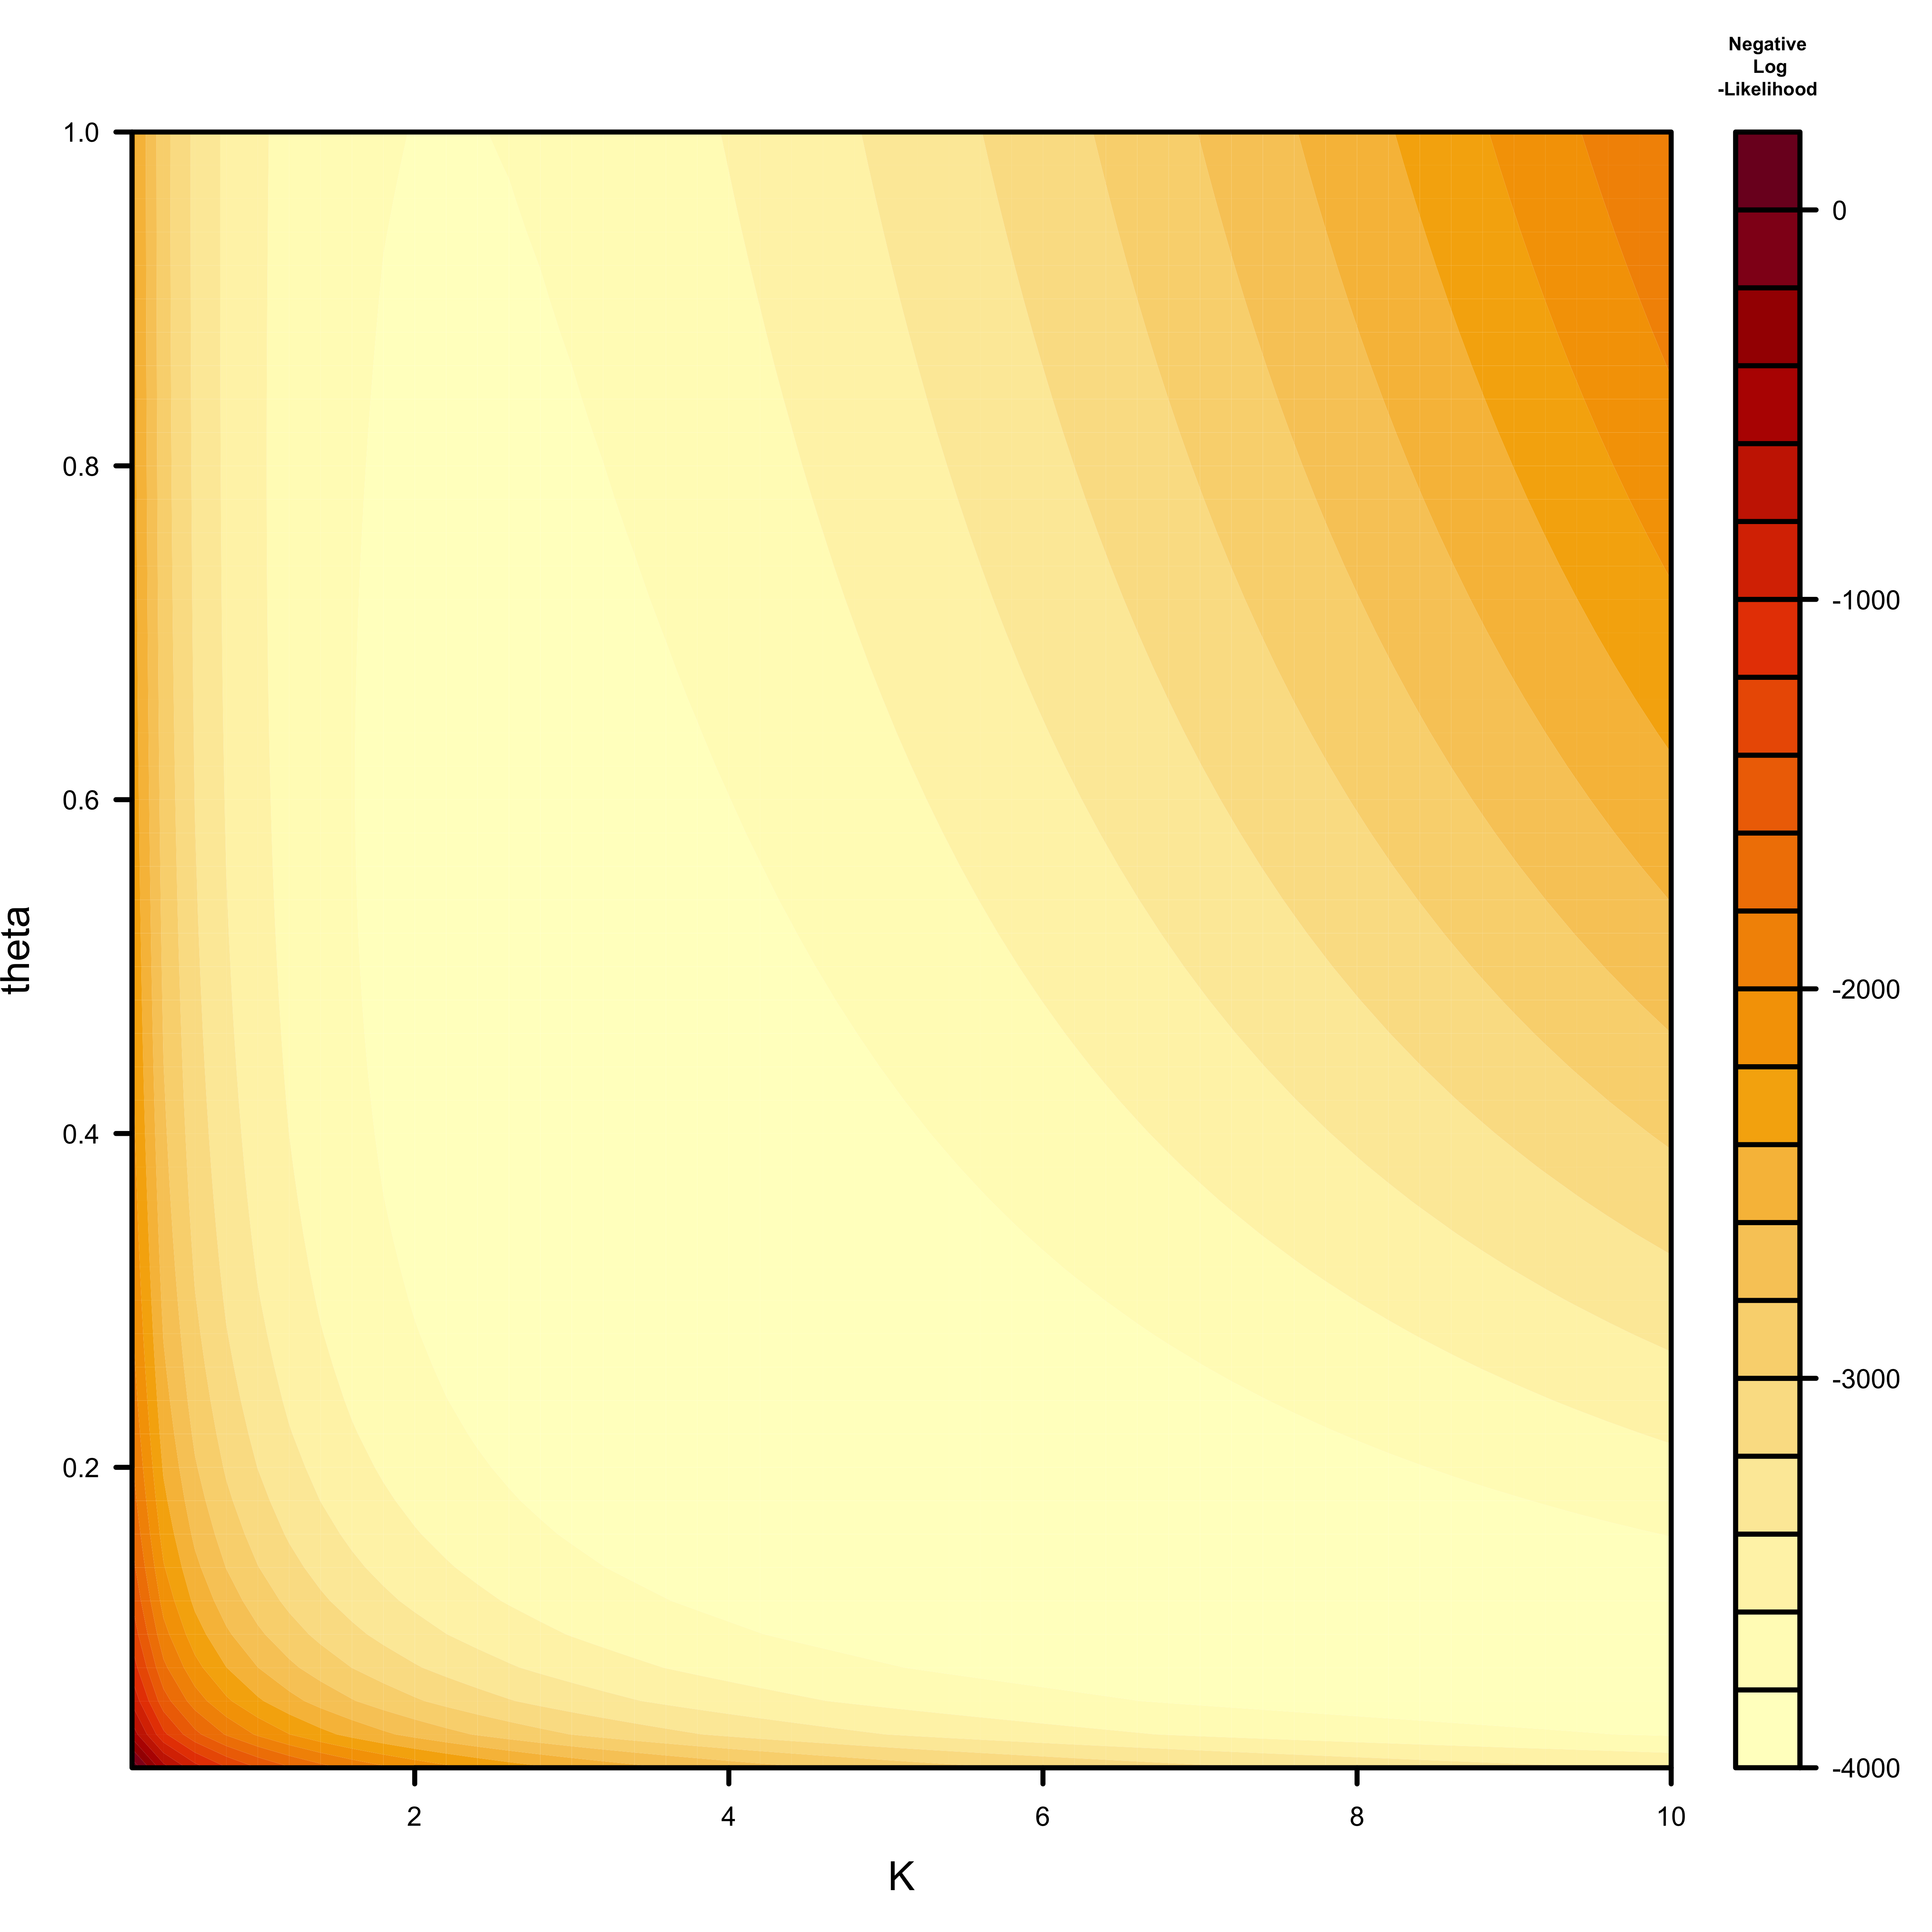
\includegraphics[width=1\linewidth]{../figures/HawkesN_contour-plot_K_theta.png}
  \caption{HawkesN}
\end{subfigure}
\caption{Contour plots of parameter negative log-likelihoods for HawkesN and SIR models. }\label{fig:contour}
\end{figure}






\begin{minipage}{\linewidth}
\centering
\captionof{table}{Table Title}\label{tab:title} 
\begin{tabular}{ C{1.25in} C{.85in} *4{C{.75in}}}\toprule[1.5pt]
\bf Variable Name & \bf Regression 1 & \bf Mean & \bf Std. Dev & \bf Min & \bf Max\\\midrule
text        &  text     & text      &  text     &  text     &text\\
\bottomrule[1.25pt]
\end {tabular}\par
\bigskip
Should be a caption
\end{minipage}


\begin{center}
\begin{tabular}{ |p{3cm}||p{1cm}|p{2.5cm}|p{1cm}|p{1cm}|p{1cm}|p{1cm}|  }
\hline
 & $I$ & $\gamma$ & $\beta$ & $K$ & $\theta$ & $c$ \\
  \hline
theoretical  & 300 & $0.2$ & 1 & 5 & 0.2 & 0.001 \\
median & 307 & $-4.3 \times 10^{-10}$ & 1.9 & 4.89 &  0.204 & 0.1 \\
sd &  11 &  $0.2$ &  1.1 & 0.52  & 0.026  & 0.000\\
 \hline
\end{tabular}
\end{center}



\section{Conclusions}




\section{Reflection}









\pagebreak

\nocite{*}

\bibliography{references}

%\bibliographystyle{plainnat}

%\section{Appendix}



%\pagebreak
%\appendix

%\begin{appendices}



%\end{appendices}

\end{document}
